\begin{savequote}[75mm]
Nulla facilisi. In vel sem. Morbi id urna in diam dignissim feugiat. Proin molestie tortor eu velit. Aliquam erat volutpat. Nullam ultrices, diam tempus vulputate egestas, eros pede varius leo.
\qauthor{Quoteauthor Lastname}
\end{savequote}

\chapter{An information-theoretic model for measuring the anonymity risk in time-variant user profiles}

\newthought{Websites and applications use personalisation services} to profile their users, collect their patterns and activities and eventually use this data to provide tailored suggestions. User preferences and social interactions are therefore aggregated and analysed. Every time a user publishes a new post or creates a link with another entity, either another user, or some on-line resource, new information is added to the user profile. Exposing private data does not only reveal information about single users' preferences, increasing their privacy risk, but can expose more about their network that single actors intended. This mechanism is self-evident on \emph{social networks} where users receive suggestions based on their friends' activity.
We propose an information theoretic approach to measure the differential update of the anonymity risk for time-varying user profiles. This expresses how privacy is affected when new content is posted and how much third party services \emph{get to know} about the users when a new activity is shared. We use real Facebook data to show how our model can be applied on a real world scenario.

\section{Background}

Personalisation and advertising services collect \emph{users} activities to provide tailored suggestions. This data contribute to form over time what is considered the user on-line footprint. With the term on-line footprint we include every possible trace left by individuals when using communication services. It follows that the same notion of digital footprint span all layers of the TCP/IP model, depending on the type of data taken into considerations. It is also important to note, that the digital footprint of an individual is formed by their interaction with their social relationships, not only their singular actions on a medium or platform.

We can therefore consider users' on-line footprints as linked data, where each event generated by a single user include information regarding other users but also regarding other events and entities. This way to consider on-line footprints is very similar to the very structure of the web, where web pages link to other pages when they reference a certain individual or object. This social and interconnected aspect of digital footprints is particularly evident for services like Facebook\cite{facebook}, where users are suggested new pages and social connections based on their friends' network of relationships and expressed preferences, or \emph{likes}.

Users' profiles also change over time, reflecting how real world individual change their tastes and preferences in comparison to, for example, a reference population. Every time new information is shared, the user is disclosing more about themselves or their social interactions, eventually changing their privacy risk.

More importantly, users tends to share their data and access to their identity accounts, such as Google~\cite{google} or Facebook~\cite{facebook}, when interacting with third party applications. These applications use federated log in mechanism through the user's identity account. To use the application, users grant it a certain level of access to their private data through their profile. This data include details about their real \emph{off-line} identity, their whereabouts and in some situations even the company they work for. Once it has gained access the application can now store user data and assume control over how it is further shared.  The  user  will never be notified again on who is accessing their data, nor if these are transferred to third parties.

This aspect of privacy protection is particularly relevant since the right to privacy is commonly interpreted as the user's right to prevent information disclosure. When a user share some content on-line, they are actively choosing to disclose some of their profile. At the same time though, they might give away more that they intended, since no information is shared from app and service provided about how the profile is analysed or how the user's data is further shared.

On-line services ask the user to access certain information, yet no concrete information is passed on how the data will be used or stored. Furthermore, these services are often designed as mobile applications where all the devices installing the  app communicate with a centralised server and constantly exchange users' information, eventually allowing for unknown third parties, or potential attackers, to fetch and store this data. In addition, this information is often shared with insecure communication through the HTTP protocol, making it possible for a malicious entity to intercept these communication and steal user data.

In this model the management of privacy and trust of the platform to which users handle their data is highly centralised. The user entrust the service with all their data, often as part of a service agreement. Generally a few services control the market and therefore can inevitably \emph{know more} about the users. This is the case of popular email or messaging services, but also social networks, relationship apps and so on. These entities can easily know who is talking to whom and sometimes also the topic of their conversations.

We analyse user on-line footprints as a series of event belonging to certain individual. Each event is a document containing different information. An event correspond to an action generated by the user or one of their devices. When a user visits a website or creates a post on a blog, an event is created. We can think of an event as a hypermedia document i.e. an object possibly containing graphics, audio, video, plain text and hyperlinks. We call the hyperlinks selectors and we use these to build the connections between the user's different identities or events. Each identity can be a profile or account that the user has created onto a service or platform, or just a collection of events, revealing something about the user. With account we mean an application account or a social network account, such as their LinkedIn or Facebook unique IDs.

When the user decide to share some new content, or subscribe a service by sharing part of their profile data, novel information is released. This information is either made public or shared to a group of people, like for a new social network post, or it is rather shared to a third party app.

We are interested to measure the differential update of the anonymity risk of user profiles due to a marginal release of novel information, based on the information-theoretic measure of anonymity risk as a Kullback-Leibler divergence between a user profile and the average population's profile.

We particularly considered real data shared by Facebook users as part of the Facebook-Tracking-Exposed project~\cite{FTE}. For the purpose of this study, we considered categorised Facebook posts. We imagined that an attacker is interested in capturing users' preferences by looking at their posts and imagined a scenario where the information shared through a new event (i.e.  sharing new content) increase or decrease the user's privacy risk, or in other world how much an attacker knows about them, once they have captured the new information.

In chapter, we build upon a recent information-theoretic model for measuring the privacy risk incurred in the disclosure of a user’s interests though on-line activity. Among other refinements, we incorporate an aspect of substantial practical importance in the aforementioned model, namely, the aspect of time-varying user profiles.

More precisely, we propose a series of refinements of a recent information-theoretic model characterising a user profile by means of a histogram of categories of interest, and measuring the corresponding privacy risk as the Kullback-Leibler divergence with respect to the histogram accounting for the interests of the overall population. Loosely speaking, this risk may be interpreted as an anonymity risk, in the sense that the interests of a specific user may diverge from those of the general population.
In this chapter, we preface our main analysis with an argument to tackle populations in which the distribution of profiles of interest is multimodal, that is, user profiles concentrate around distinguishable clusters of archetypical interests. We suggest that said information-theoretic model be applied after segmentation of the overall population according to demographic factors, effectively extending the feasibility of the original, unimodal proposal.

Then, we introduce the most important refinement and undoubtedly the main focus of this chapter, consisting in the extension of the aforementioned model to time-varying user profiles. Despite the practical significance of the aspect of time in the analysis of privacy risks derived from disclosed on-line activity, it is nevertheless an aspect all too often neglected, which we strive to remedy with this preliminary proposal. Here, the time variation addresses not only changes over time in the interests of a user, construed as a dynamic profile, but also novel activity of a possibly static profile, only partially known in practice.

The changes in anonymity risk are formulated as a gradient of the Kullback-Leibler divergence of a user profile reflecting newly observed activity, with respect to a past history, and are inspired in the abstract formulation of Bregman projections onto convex sets, whose application to the field of privacy is, to the best of our knowledge, entirely novel.

For a given activity and history, we investigate the profile updates leading to the best and worst overall anonymity risk, and connect the best case to the fairly recent information-theoretic framework of optimised query forgery and tag suppression for privacy protection.

We contemplate certain special cases of interest. On the one hand, we provide a corollary of our analysis for the special case in which the anonymity risk is measured as the Shannon entropy of the user profile. On the other hand, we particularise our model in the extreme case in which the new observation consists in a single sample of categorised on-line activity.

Last but not least, we verify and illustrate our model with a series of examples and experiments with both synthetic and real on-line activity.

\section{An information\hyp theoretic model for measuring anonymity risk}
\label{sec:1.1}
Consider a user profile $p$, together with an average population profile $q$, both represented as histograms of relative frequencies of on-line activity along predefined categories of interest $i=1,\dots,m$. In the absence of a specific statistical model on the frequency distribution of user profiles, as argued extensively in~\cite{Rebollo10IT, Rebollo11SecTech, Parra14FGCS} on the basis of Jaynes' rationale for maximum entropy methods, we assume that the \emph{anonymity risk} may be adequately measured as the \emph{Kullback\hyp Leibler} (KL) \emph{divergence} $\text{D}(p\|q)$ between the user profile $p$ and the population's~$q$. The idea is that user profiles become less common as they diverge from the average of the population. Precisely, we define the anonymity risk as
$$\mathcal{R}\defeq\text{D}(p\|q)\defeq\sum_{i=1}^m p_i\log \frac{p_i}{q_i}.$$
Usually, the basis of logarithm is 2 and the units of the divergence are bits.

Intuitively, the empirical histogram of relative frequencies (or type) $t$ of $n$ independent, identically distributed drawings should approach the true distribution $\bar{t}$ as $n$ increases. Those drawing may be loosely interpreted as sequences of online queries according to some underlying user interests represented by~$\bar{t}$. More technically, the extension of Jaynes' approximation to KL divergences for a sequence of independent shows that the probability $p_T(t)$ of the empirical distribution $t$ is related to the KL divergence $\text{D}(t\|\bar{t})$ with respect to the true distribution $\bar{t}$ by means of the limit
$$-\tfrac{1}{n}\log p_T(t)\xrightarrow[n\to\infty]{}\text{D}(t\|\bar{t}).$$

According to this model, the user profile $p$ plays the role of the empirical distribution $t$, and the population's profile $q$, the role of the true distribution~$\bar{t}$. In a way, we construe a user profile as an empirical instantiation of the population's profile. Concordantly, the divergence $\text{D}(p\|q)$ between the user profile $p$ and the population's $q$ is a measure of how rare $p$ should be, which we regard as a measure of \emph{anonymity risk}. The argument that the rarity of a profile may also be understood as a measure of how sensitive a user profile may be considered, offers a measure of \emph{privacy risk}. Admittedly, this model is limited to applications where the underlying assumptions may be deemed adequate, particularly when no specific, possibly multimodal distribution of the user profiles is available.

Another helpful interpretation of this measure stems from rewriting the user profile as a distribution $p_{I|J}$ of a random variable $I$ indexing on-line activity into predefined categories $i=1,\dots,m$, conditioned on the user identity $J$, defined on the user indexes $j=1,\dots,n$. Observing that the population profile is the expectation across all user profiles,
$$q_I=\text{E}_J\:p_{I|J}(\cdot|J),\quad\text{(more explicitly},\quad q_I(i)=\tfrac{1}{n}\sum_{j=1}^n p_{I|J}(i|j)\quad\text{for all}\ i\text{)},$$
we immediately conclude that the expected risk is
$$\text{E}_J\:\mathcal{R}(J)=\text{E}_J\:\text{D}\left(p_{I|J}(\cdot|J)\,\middle\|\,q_I\right)=\text{I}(I;J),$$
namely, the mutual information between the on-line activity $I$ and the user identity~$J$.

\subsection{Multimodality of the KL divergence model and conditioning on demography}
\label{sec:1.2}
Perhaps one of the major limitations of the direct application of the KL divergence model for characterising the anonymity of a profile is made clear when the distribution of profiles is concentrated around several predominant modes, contradicting the implicit unimodal assumption revolving around the population's profile~$q$. Intuitively, one may expect several clusters in which profiles are concentrated, corresponding to various demographic groups, characterised by sex, age, cultural background, etc.

In order to work around this apparent limitation, we may simply partition the data into a number of meaningful demographic groups, indexed by $k$, and calculate the average population profile $q_{I|K}(\cdot|k)$ for each group~$k$. Then, redefine the demographically contextualised anonymity risk as the KL divergence between the profile $p_{I|J}(\cdot|j)$ of user $j$, in group $k(j)$, and the corresponding reference $q_{I|K}(\cdot|k(j))$, that is,
$$\mathcal{R}_\text{context}(j)\defeq\text{D}\left(p_{I|J}(\cdot|j)\,\middle\|\,q_{I|K}(\cdot|k(j))\right).$$
Obviously, the model will be suitable as long as the profile distribution is unimodal within each demographic context, in the absence of a more specific model. Note that the measure of anonymity risk of the disclosed interests is now conditioned on demographic data potentially observable by a privacy attacker.

\subsection{Gradient of the KL divergence and information projection}
\label{sec:1.3}

\noindent
Before addressing the problem of the differential update per se, we quickly review an interesting result on the gradient of the KL divergence, and its application to convex projections with said divergence. Directly from the definition of the KL divergence between distributions $p$ and $q$ for a general logarithmic basis, compute the gradient on the first argument
$$\nabla_p\text{D}(p\|q)={\left(\log \frac{p_i}{q_i}+\log e\right)}_i.$$
Swift algebraic manipulation shows that
$$\text{D}(p\|q)=\text{D}(p\|p^*)+\text{D}(p^*\|q)+\nabla_{p^*}\text{D}(p^*\|q)^\text{T}(p-p^*),$$
for any additional distribution $p^*$, where the constant term $\log e$ in the gradient becomes superfluous, on account of the fact that $\sum_i p_i-p_i^*=0$. Observe that part of the above expression may be readily interpreted as the Taylor expansion of $\text{D}(p\|q)$ about $p^*$,
$$\text{D}(p\|q)=\text{D}(p^*\|q)+\nabla_{p^*}\text{D}(p^*\|q)^\text{T}(p-p^*)+O(\|p-p^*\|^2),$$
with error precisely $\text{D}(p\|p^*)$.

\begin{figure}[htb]
\centering
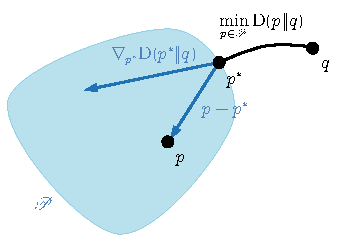
\includegraphics[scale=\FigScale]{figures/ConvProj.pdf}
\caption{Information projection $p^*$ of a reference distribution $q$ onto a convex set~$\mathscr{P}$.}
\label{fig:1}
\end{figure}

In the context of convex projections, suppose that we wish to find the closest point $p^*$ inside a convex set $\mathscr{P}$ to a reference point $q$, in KL divergence, succinctly,
$$p^*=\operatorname*{arg\,min}_{p\in\mathscr{P}} \text{D}(p\|q).$$
This problem is represented in Fig.~\ref{fig:1}. The solution $p^*$ is called the \emph{information projection} of $q$ onto $\mathscr{P}$. Because for such $p^*$ the projection of the gradient of the objective onto the vector difference $p-p^*$ for any $p\in\mathscr{P}$ must be nonnegative, i.e.,
$$\nabla_{p^*}\text{D}(p^*\|q)^\text{T}(p-p^*)\geqslant 0,$$
we may conclude from the previous equality involving the gradient that
$$\text{D}(p\|q)\geqslant\text{D}(p\|p^*)+\text{D}(p^*\|q).$$
This last inequality is, in fact, a known generalisation of the Pythagorean theorem for projections onto convex sets, generally involving obtuse triangles\footnote{The expression relating the gradient with a set of divergences shown here may be readily generalise to prove an analogue of the Pythagorean theorem for Bregman projections. Recall that Bregman divergences encompass both squared Euclidean distances and KL divergences as a special case. An alternative proof of the Pythagoream theorem for KL divergences, which inspired a small part of the analysis in this manuscript, can be found in \cite{cover91b}(Theor.~11.6.1).}.

\begin{figure}[htb]
\centering
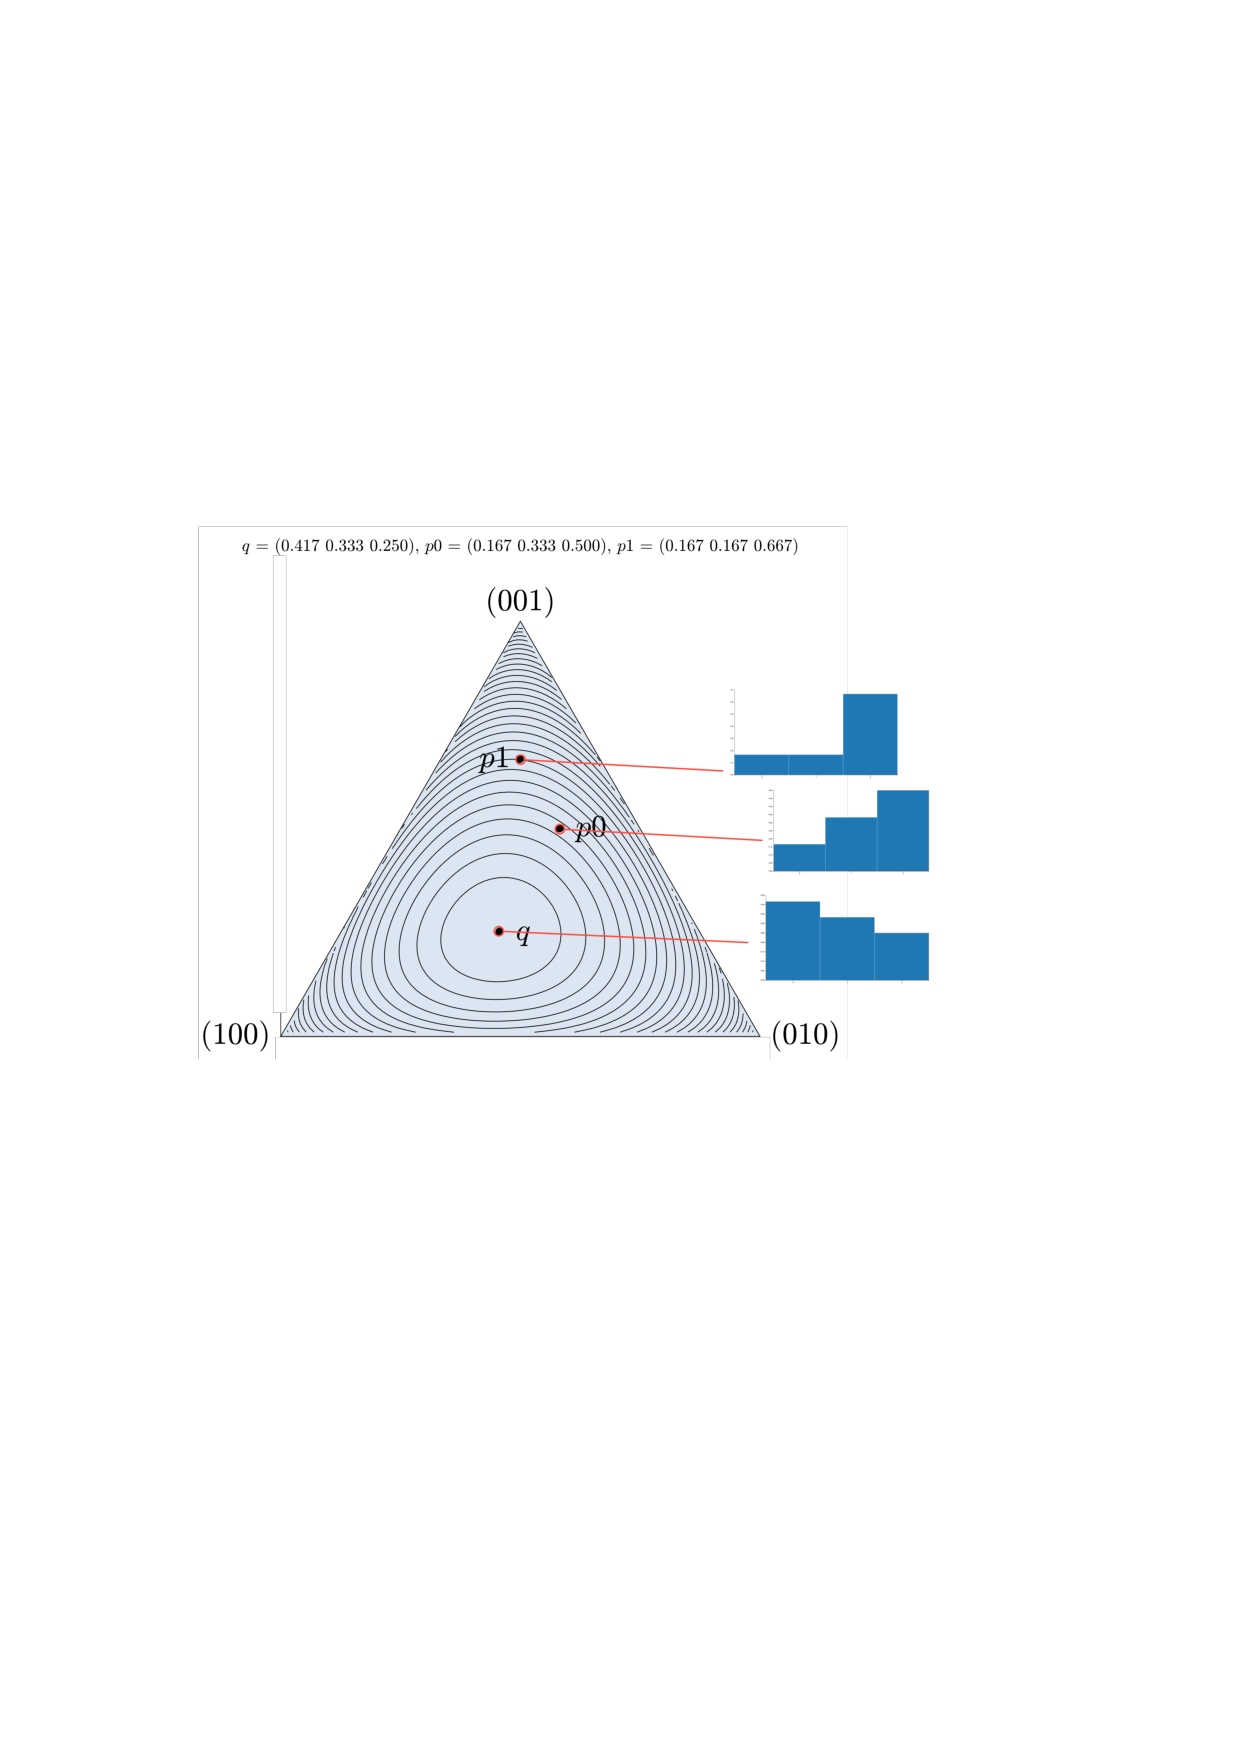
\includegraphics[scale=0.5]{figures/triplex_profiles.pdf}
\caption{Probability simplices showing, the population distribution $q$, the user's profile $p_0$, the updated profile $p_1$.}
\label{fig:2-1}
\end{figure}

\subsection{Differential update of the anonymity risk due to revealing new information}
\label{sec:1.4}

\noindent
Under this simple model, we consider the following problem. Suppose that the distribution $p_0$ represents a history of on-line activity of a given user up to this time, with associated anonymity risk $\text{D}(p_0\|q)$. Consider now a series of new queries, with interests matching a profile $p_1$ and associated risk $\text{D}(p_1\|q)$~\ref{fig:2-1}. If those new queries were observed, the overall user profile would be updated to
$$p_\alpha = (1-\alpha)p_0+\alpha p_1,$$~\ref{fig:2-2}
where the activity parameter $\alpha\in(0,1)$ is the fraction of new queries with respect to the total amount of queries released. We investigate the updated anonymity risk
$$\text{D}((1-\alpha)p_0+\alpha p_1\|q)$$
in terms of the risks associated with the past and current activity, for a marginal activity increment~$\alpha$. To this end, we analyse the first argument of the KL divergence, in the form of a convex combination, through a series of quick preliminary lemmas\footnote{The mathematical proofs and results developed here may be generalised in their entirety from KL divergences to Bregman divergences, and they are loosely inspired by a fundamental Pythagorean inequality for Bregman projections on convex sets.}.

\begin{figure}[htb]
\centering
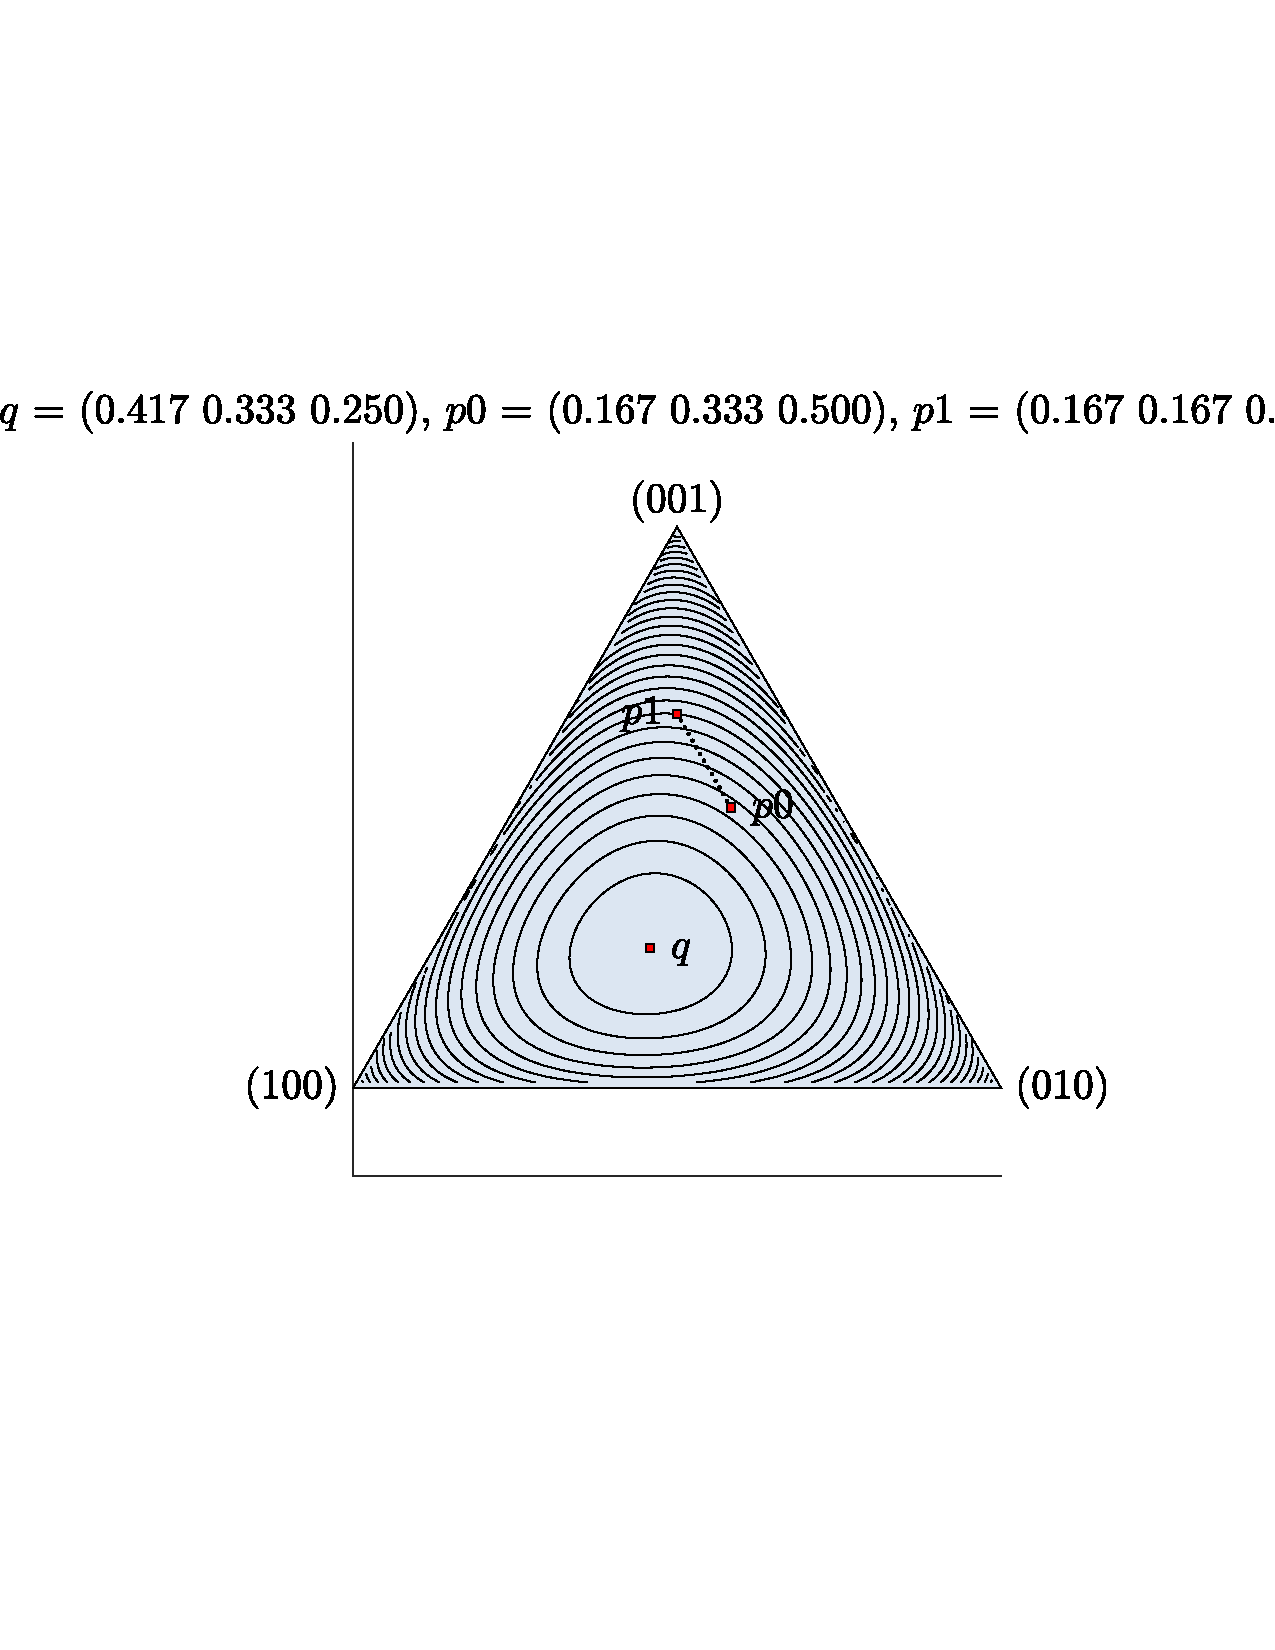
\includegraphics[scale=0.5]{figures/triplex_alpha.pdf}
\caption{Probability simplices showing, the population distribution $q$, the user's profile $p_0$, the updated profile $p_1$. The intermediate points show the value of $p_\alpha$ for different $\alpha$ }
\label{fig:2-2}
\end{figure}

On the one hand, since the KL divergence is a convex function, we may bound the updated risk as
$$\text{D}\left((1-\alpha)p_0+\alpha p_1\middle\|q\right)\leqslant(1-\alpha)\text{D}(p_0\|q)+\alpha\,\text{D}(p_1\|q).$$
On the other hand, we may resort to our previous gradient analysis in \S \ref{sec:1.3} to write the first\hyp order Taylor approximation
$$\text{D}\left((1-\alpha)p_0+\alpha p_1\middle\|q\right)=(1-\alpha)\text{D}(p_0\|q)+\alpha\,\text{D}(p_1\|q)-\alpha\,\text{D}(p_1\|p_0)+O(\alpha^2).$$

This last expression is consistent with the convexity bound, and quite intuitively, the term $-\alpha\,\text{D}(p_1\|p_0)$ in the Taylor approximation refining the convex bound vanishes for negligible activity $\alpha$ or new activity profile $p_1$ similar to the history $p_0$ revealed thus far. We may alternatively write the updated risk as an increment with respect to that based on the user's on-line history, as
$$\text{D}\left((1-\alpha)p_0+\alpha p_1\middle\|q\right)-\text{D}(p_0\|q)=\alpha\left(\text{D}(p_1\|q)-\text{D}(p_0\|q)-\text{D}(p_1\|p_0)\right)+O(\alpha^2),$$
which we observe to be approximately proportional to the relative activity parameter $\alpha$, and to an expression that only depends on the divergences between the profiles involved.

\subsection{Special cases of delta update and uniform reference}
\label{sec:1.5}

\noindent
In the special case when the new activity contains a single query, the new profile $p_1$ is a Kronecker delta $\delta^i$ at some category~$i$. In this case,
$$\text{D}(p_1\|q)=\text{D}(\delta^i\|q)=-\log q_i,\ \text{and}$$
$$\text{D}\left((1-\alpha)p_0+\alpha p_1\middle\|q\right)=(1-\alpha)\text{D}(p_0\|q)+\alpha\log \frac{p_{0\,i}}{q_i}+O(\alpha^2).$$
A second corollary follows from taking the reference profile $q$ as the uniform distribution $u=\tfrac{1}{m}$, and replacing KL divergences with Shannon entropies according to
$$\text{D}(p\|u)=\log m-\text{H}(p).$$
Precisely,
$$\text{H}\left((1-\alpha)p_0+\alpha p_1\right)\geqslant(1-\alpha)\text{H}(p_0)+\alpha\,\text{H}(p_1).$$
consistently with the concavity of the entropy, and
$$\text{H}\left((1-\alpha)p_0+\alpha p_1\right)=(1-\alpha)\text{H}(p_0)+\alpha\,\text{H}(p_1)+\alpha\,\text{D}(p_1\|p_0)+O(\alpha^2).$$
Even more specifically, in the case of a delta update $p_1=\delta^i$ and uniform reference profile,
$$\text{H}\left((1-\alpha)p_0+\alpha p_1\right)=(1-\alpha)\text{H}(p_0)-\alpha\log p_{0\,i}+O(\alpha^2).$$

\subsection{Best and Worst Update}
\label{sec:1.6}

\noindent
For a given activity $\alpha$ and history $p_0$, we investigate the profile updates $p_1$ leading to the best and worst overall anonymity risk $\text{D}\left((1-\alpha)p_0+\alpha p_1\middle\|q\right)$. The problem of finding the best profile, yielding the smallest risk, is formally identical to that of optimal query forgery extensively analysed in~\cite{Rebollo10IT}. Note that this problem may also be interpreted as the information projection of the population profile $q$ onto the convex set of possible forged profiles
$$\mathscr{P}=\left\{(1-\alpha)p_0+\alpha p_1\right\},$$
with fixed $\alpha$ and $p_0$, a scaled, translated probability simplex. In this case, the generalized Pythagorean theorem shown earlier guarantees
$$\text{D}\left((1-\alpha)p_0+\alpha p_1\middle\|q\right)\geqslant\text{D}\left((1-\alpha)p_0+\alpha p_1^*\middle\|(1-\alpha)p_0+\alpha p_1\right)+\text{D}\left((1-\alpha)p_0+\alpha p_1^*\middle\|q\right).$$

We may now turn to the case of the worst profile update $p_1$, leading to the highest anonymity risk. Consider two distributions $p$ and $q$ on the discrete support alphabet $i=1,\dots,m$, representing predefined categories of interest in our context. Recall that $p$ is said to be \emph{absolutely continuous} with respect to $q$, denoted $p\ll q$, whenever $q_i=0$ implies $p_i=0$ for each~$i$. Otherwise, if for some $i$, we had $p_i>0$ but $q_i=0$, then $\text{D}(p\|q)=\infty$. In the context at hand, we may assume that the population profile incorporates all categories of interest, so that $q_i>0$, which ensures absolute continuity, i.e., $p\ll q$. Therefore, we would like to solve
$$\max_{p_1\ll q} \text{D}\left((1-\alpha)p_0+\alpha p_1\middle\|q\right).$$

We shall distinguish two special cases, and leave the general maximisation problem for future investigation. Let us tackle first the simpler case $\alpha=1$, and call $p_1=p$. Recall that the \emph{cross\hyp entropy} between two distributions $p$ and $q$ is defined as
$$\text{H}(p\|q)=-\sum_{i=1}^m p_i\log q_i,$$
and is related to the (Shannon) entropy and the KL divergence via
$$\text{H}(p\|q)=\text{H}(p)+\text{D}(p\|q).$$
Clearly,
$$\max_{p\ll q} \text{H}(p\|q)=-\log q_\text{min},$$
attained for $p=\delta^i$ corresponding to the category $i$ minimising~$q$. It turns out that this is also the solution to the maximisation problem in the divergence, because
$$\text{D}(p\|q)=\text{H}(p\|q)-\text{H}(p),$$
and $\text{H}(\delta^i)=0$, which means that $p=\delta^i$ simultaneously maximises the cross\hyp entropy and minimises the entropy.

The second special case we aim to solve is that of a uniform reference $q=u$, discussed in \S \ref{sec:1.5}. The corresponding problem is
$$\min_{p_1} \text{H}\left((1-\alpha)p_0+\alpha p_1\right).$$
We claim that the worst profile update $p_1$ is again a Kronecker delta, but this time at the category $i$ maximising $p_0$. Indeed, assume without loss of generality that $p_0$ is sorted in decreasing order, observe that $(1-\alpha)p_0+\alpha\delta^1$ majorises any other convex combination $(1-\alpha)p_0+\alpha p_1$, and recall that the entropy is Schur\hyp concave.

As for the general case, the associated cross\hyp entropy problem is fairly simple. We have
$$\max_{p_1\ll q} \text{H}\left((1-\alpha)p_0+\alpha p_1\middle\|q\right)=(1-\alpha)\text{H}(p_0\|q)-\alpha\log q_\text{min},$$
for $p=\delta^i$ at the category minimising~$q$. Unfortunately, the terms in the difference
$$\text{D}\left((1-\alpha)p_0+\alpha p_1\middle\|q\right)=\text{H}\left((1-\alpha)p_0+\alpha p_1\middle\|q\right)-\text{H}\left((1-\alpha)p_0+\alpha p_1\right),$$
are respectively maximised and minimised for deltas at different categories, in general, namely that minimising $q$, and that maximising $p_0$. We may however provide an upper bound on the anonymity risk based on these considerations; by virtue of the convexity of the divergence and the previous result on its maximisation,
$$\text{D}\left((1-\alpha)p_0+\alpha p_1\middle\|q\right)\leqslant(1-\alpha)\text{D}(p_0\|q)-\alpha\log q_\text{min}.$$


%%%%%%%%%%%%%%%%%%%%%%%%%%%%%%%%%%%%%%%%%%

\section{Results and discussion}

In the previous section, we formulated the theoretical problem of the differential update of the anonymity risk of time-varying user profiles due to a marginal release of novel information, based on the information\hyp theoretic measure of anonymity risk as a Kullback\hyp Leibler divergence between a user profile and the average population's profile. In this section, we apply the theoretical conclusions drawn in previous sections.

\subsection{Examples}

We have stated in \S \ref{sec:1.4} that the KL divergence is a convex function. We now consider a scenario where a user is sharing some new information and wants to find what is their updated privacy risk.

\begin{figure}[htb]
\centering
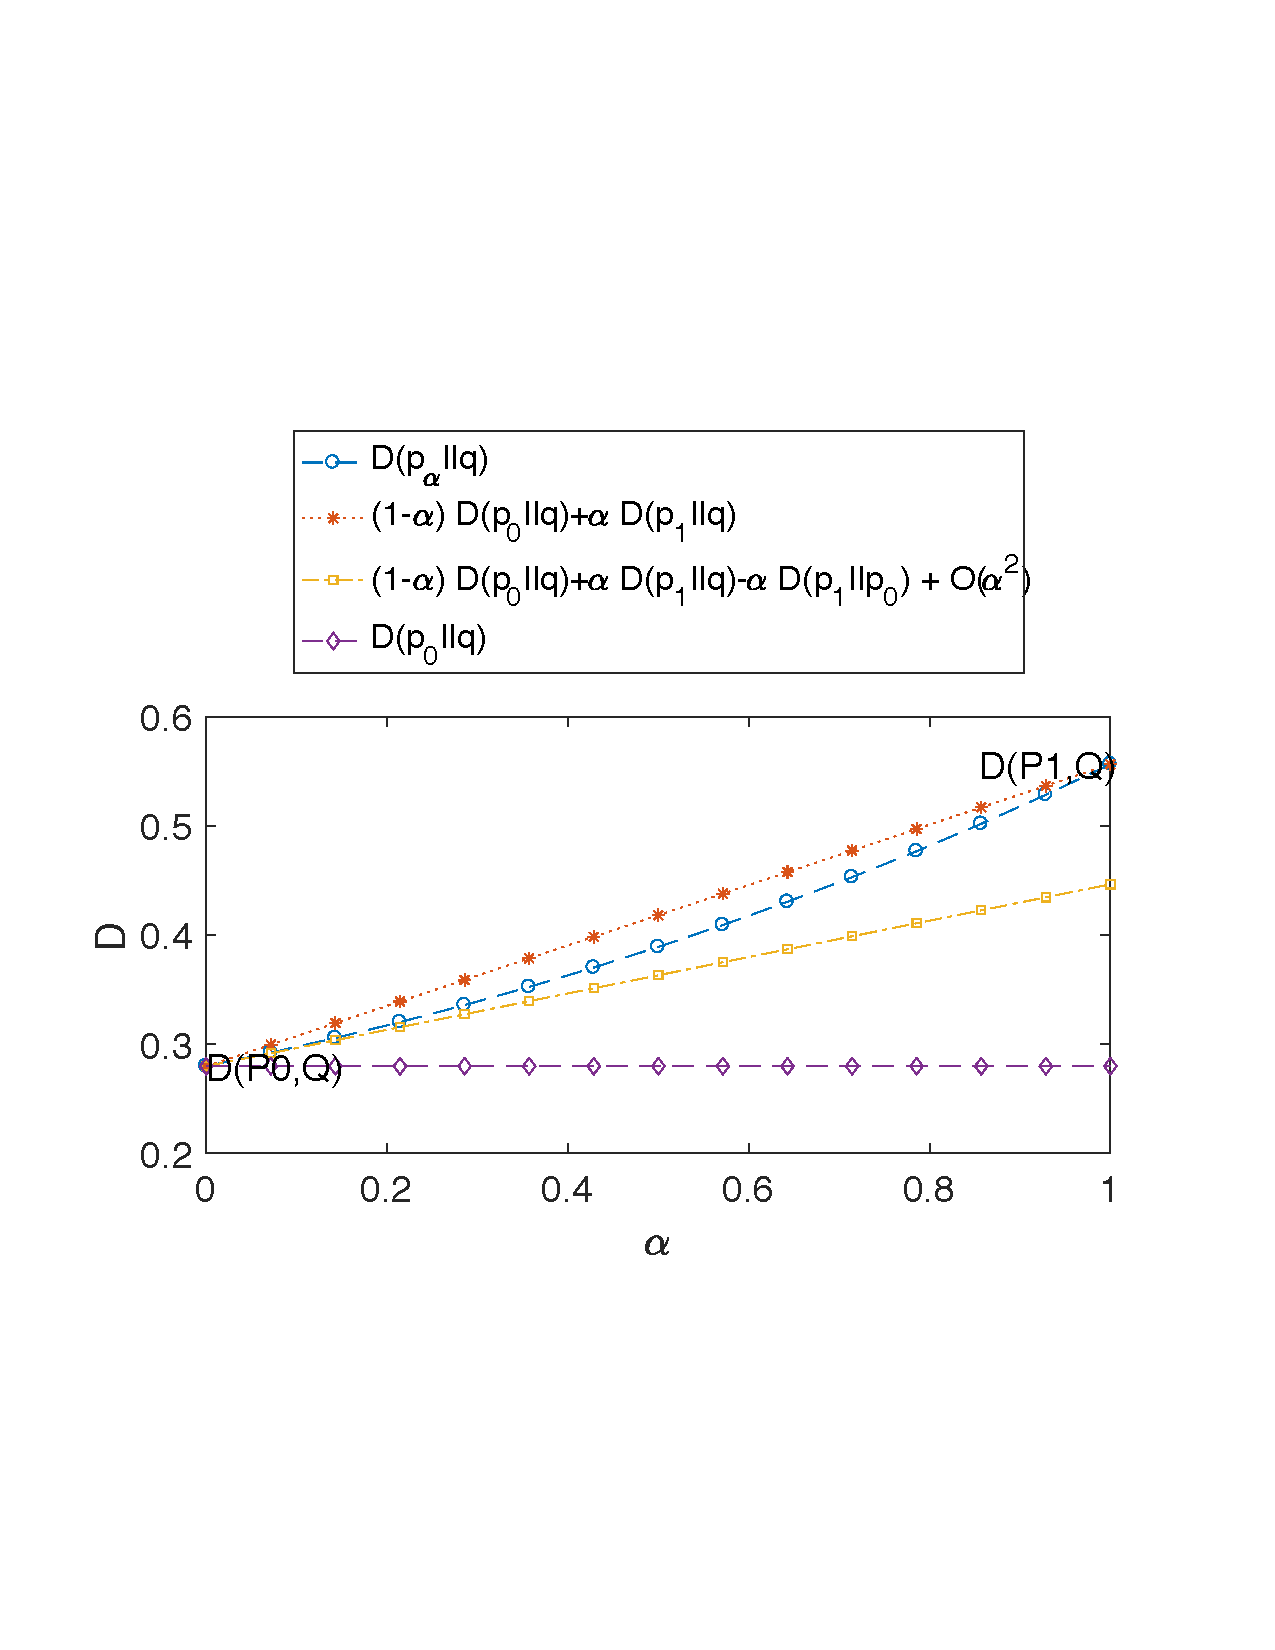
\includegraphics[scale=0.5]{figures/example_1_D.pdf}
\caption{Privacy risk $D$ between a user's profile $p$ and reference distribution $q$.}
\label{fig:3}
\end{figure}

We show how the updated privacy risk $\text{D}\left((1-\alpha)p_0+\alpha p_1\middle\|q\right)$ is bounded by: $(1-\alpha)\text{D}(p_0\|q)+\alpha\,\text{D}(p_1\|q).$ (Figure: ~\ref{fig:3}). For the Shannon Entropy we show the symmetrical result for which the updated risk $\text{H}\left((1-\alpha)p_0+\alpha p_1\right)$ bounds $(1-\alpha)\text{H}(p_0)+\alpha\,\text{H}(p_1).$ (Figure: ~\ref{fig:4}).

\begin{figure}[htb]
\centering
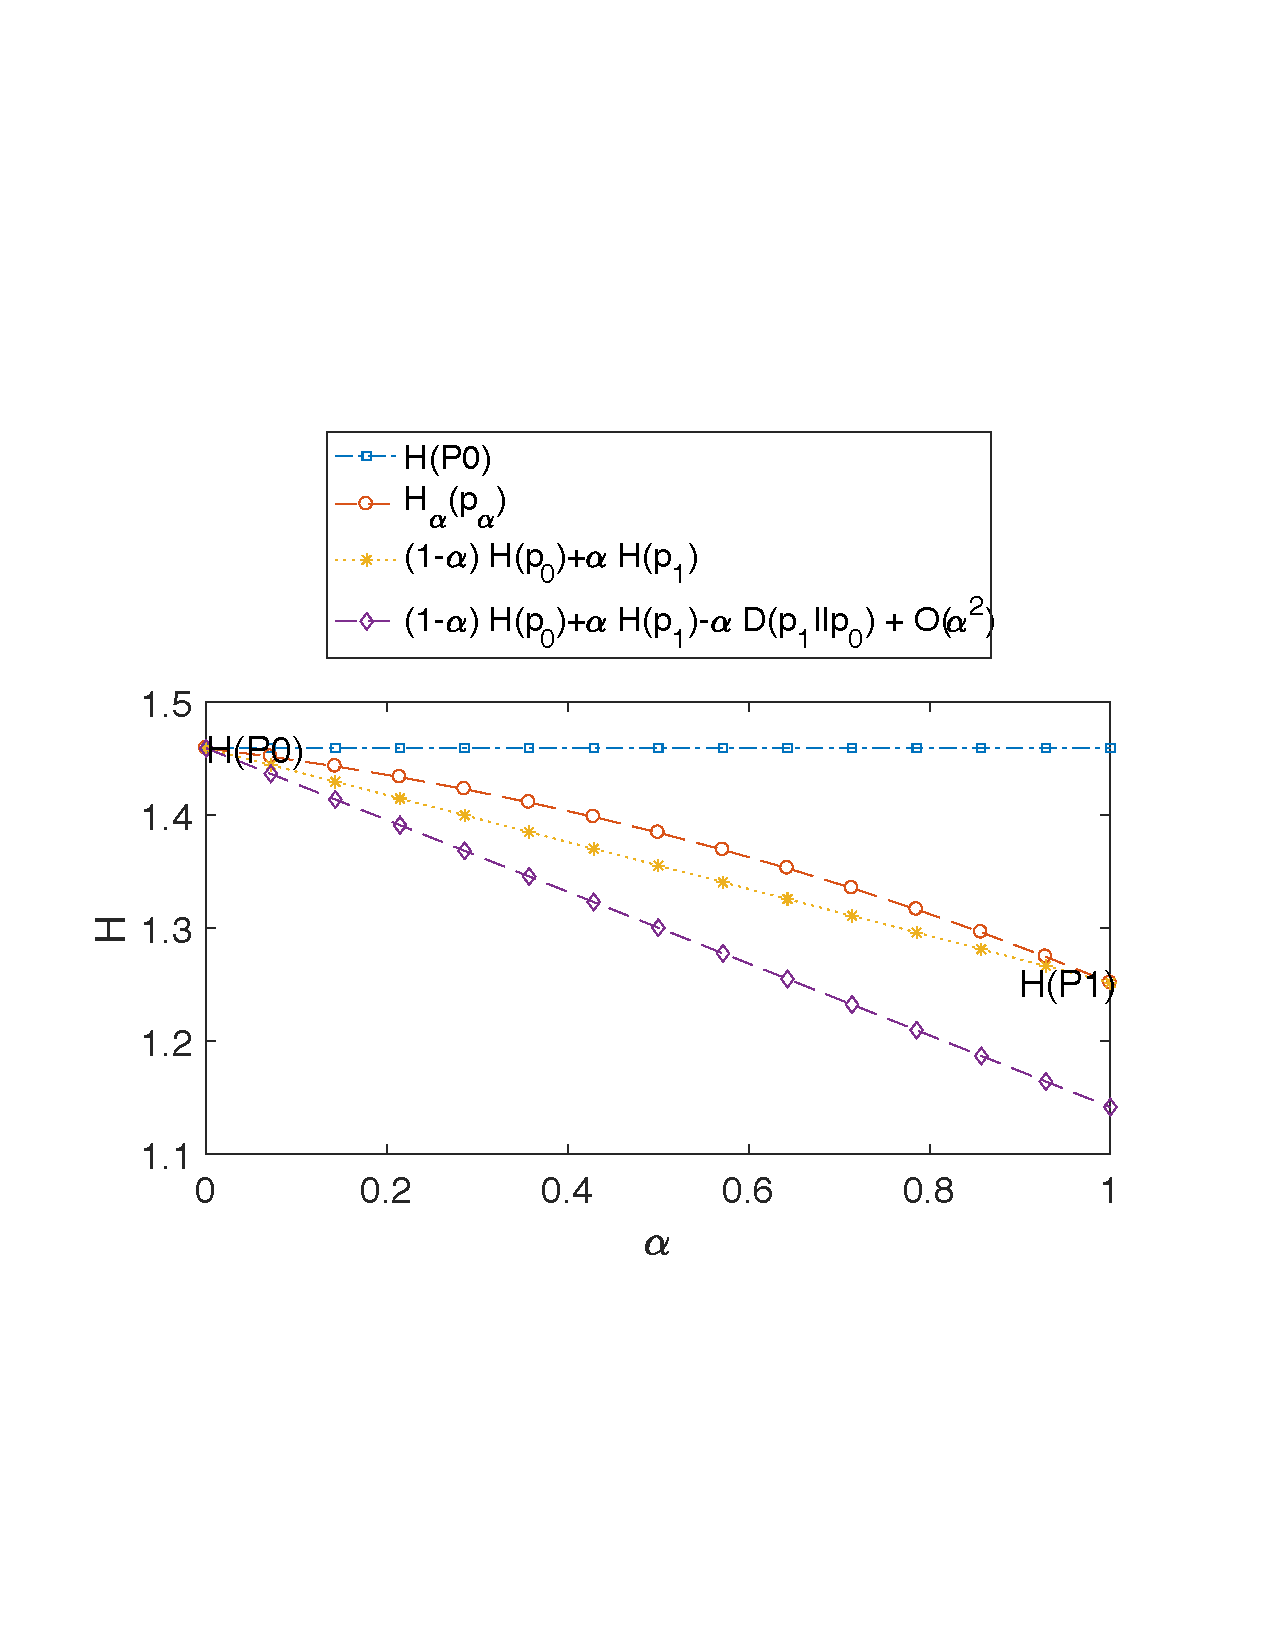
\includegraphics[scale=0.5]{figures/example_1_H.pdf}
\caption{Entropy $H$ for a user's profile $p$.}
\label{fig:4}
\end{figure}

We now present, for a given activity $\alpha$ fixed, and given history $p_0$ the profile updates $p_1$ leading to the best and worst overall anonymity risk (\S  \ref{sec:1.6}). We illustrate this both for privacy risk based on the KL-Divergence (Figure: ~\ref{fig:5}) and for the Shannon entropy (Figure: ~\ref{fig:6}). The user and population profiles are, in this case, synthetic.

\begin{figure}[htb]
\centering
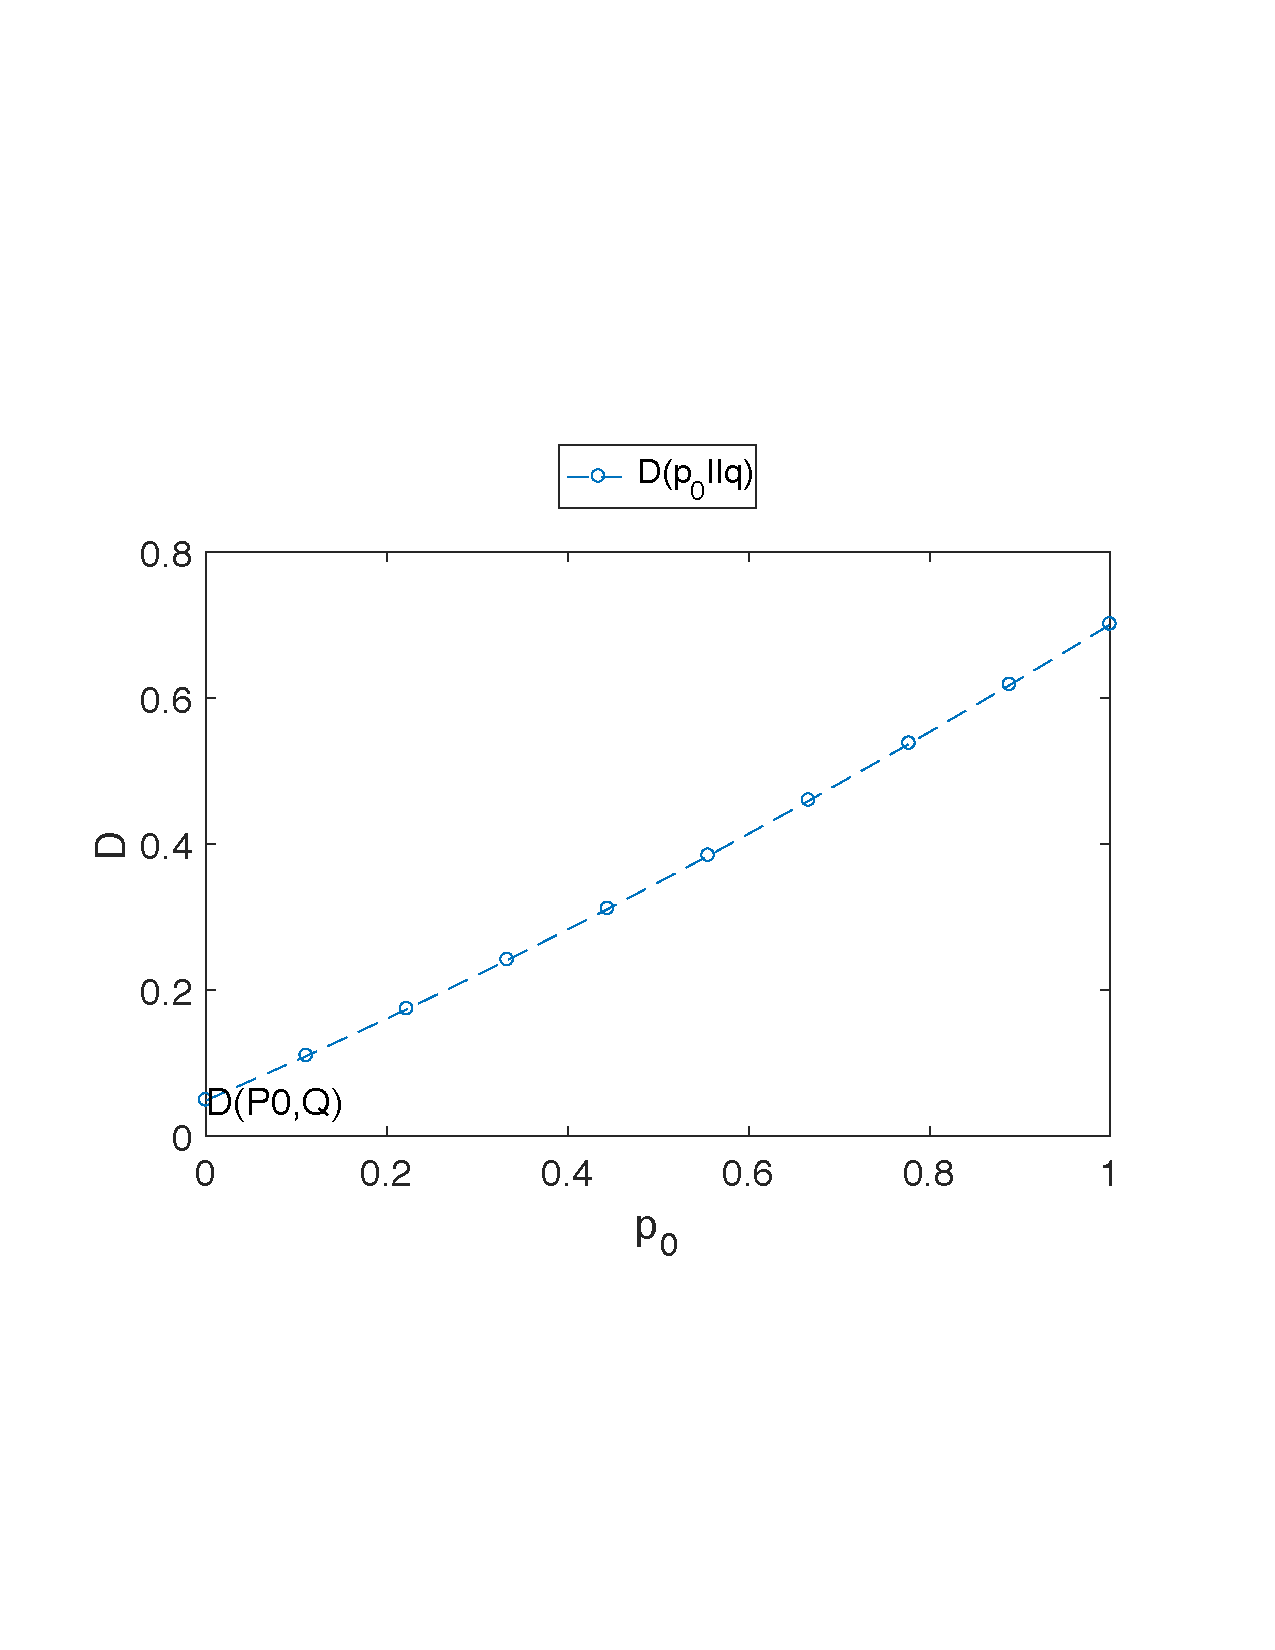
\includegraphics[scale=0.5]{figures/example_2_D.pdf}
\caption{Privacy risk $D$ between a user's profile $p$ and reference distribution $q$.}
\label{fig:5}
\end{figure}

\begin{figure}[htb]
\centering
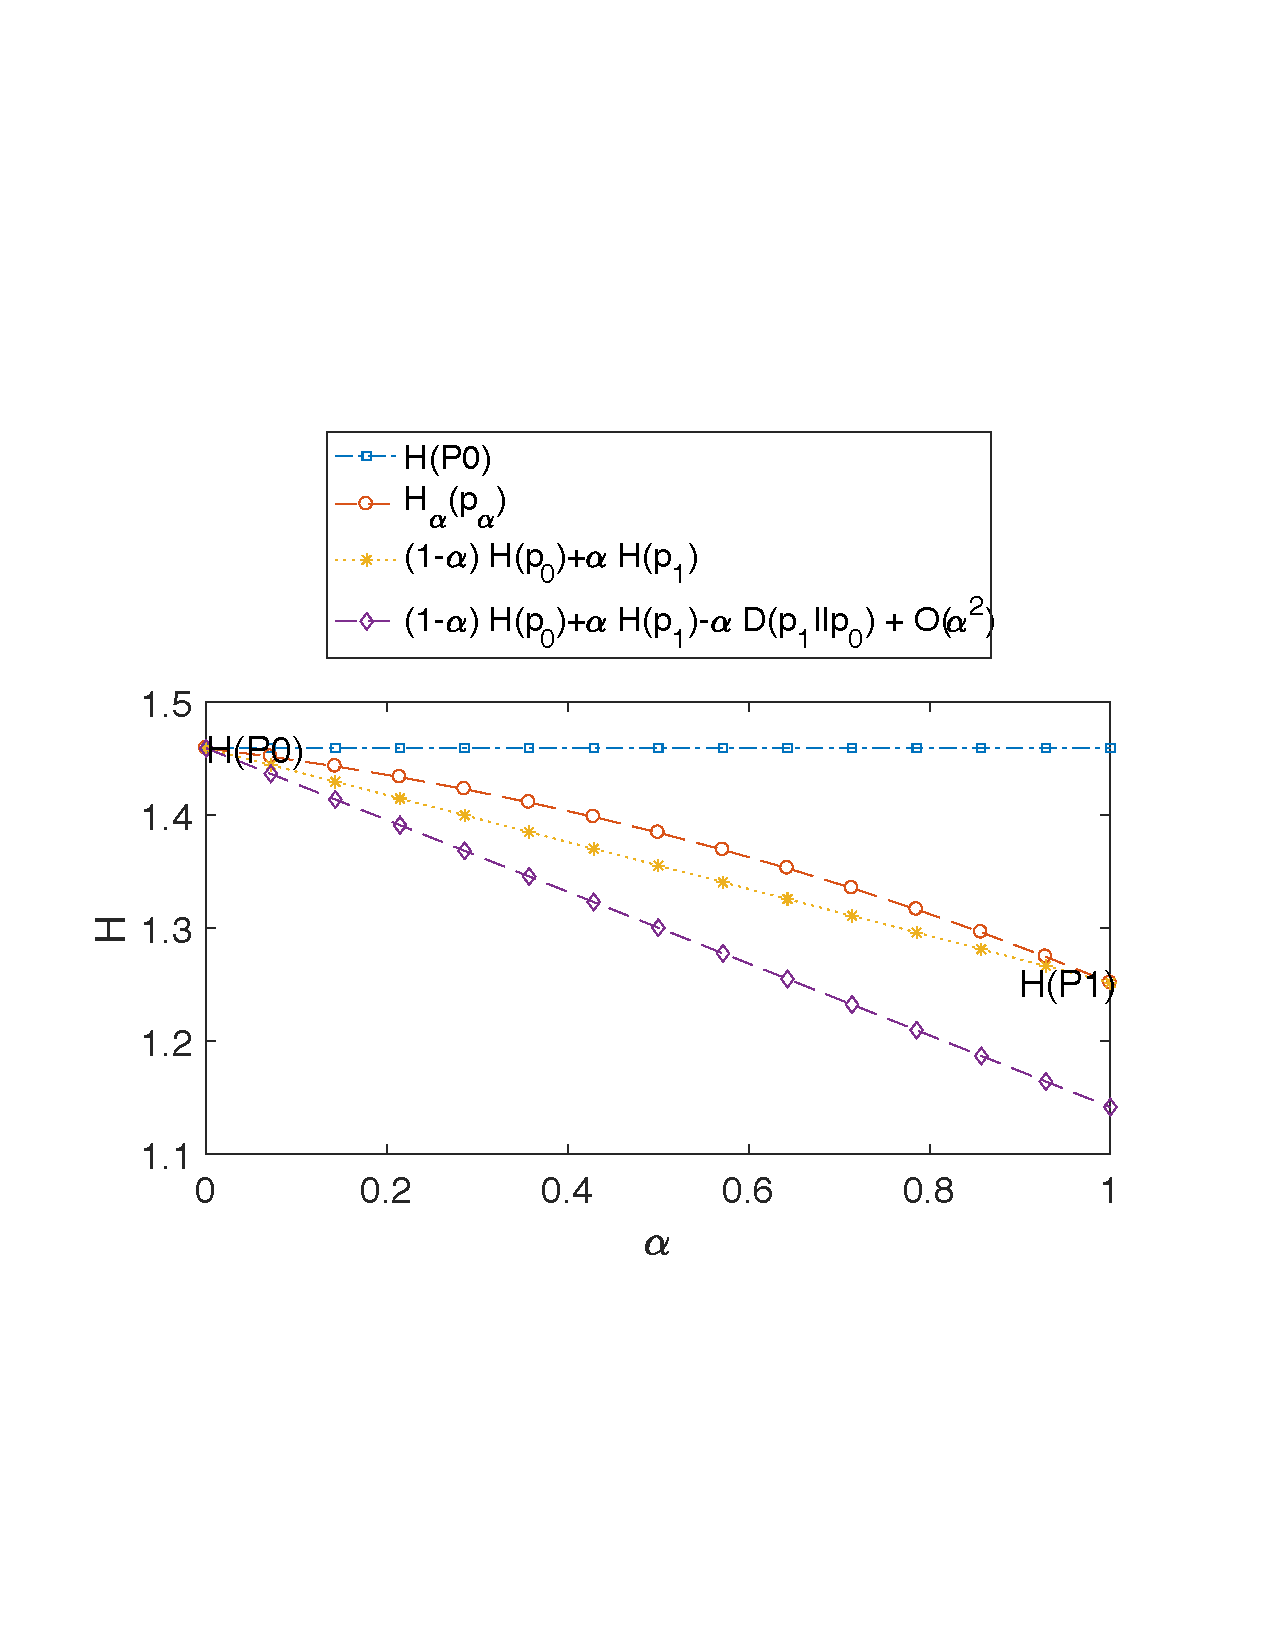
\includegraphics[scale=0.5]{figures/example_1_H.pdf}
\caption{Entropy $H$ for a user's profile $p$.}
\label{fig:6}
\end{figure}

\subsection{Results}

We consider now a scenario for which a population of users sharing posts on Facebook. For the purpose of this study we have used data extracted from the Facebook-Tracking-Exposed project~\cite{FTE}, where users contribute their data to gain more insights on Facebook personalisation algorithm.

The extracted dataset contained 59188 posts of 4975 timelines. We consider a series 376 of shared posts of a single user. For a fixed history of 361 posts we considered a sliding window over 15 posts overtime, to capture how a profile changes over time.

We considered the privacy risk between a user's profile $p$ in the Facebook dataset and reference population distribution $q$ (Figure: ~\ref{fig:7}). Furthermore we considered the $\delta \mathcal{R} = \text{D}(p_\alpha\|q) - \text{D}(p_0\|q)$. Recall that $p_0$ is a user's profile in the Facebook dataset, built taking into consideration a long series of samples. Instead, $q$ is the reference population distribution calculated for all the posts in the dataset (Figure: ~\ref{fig:8}).

\begin{figure}[htb]
\centering
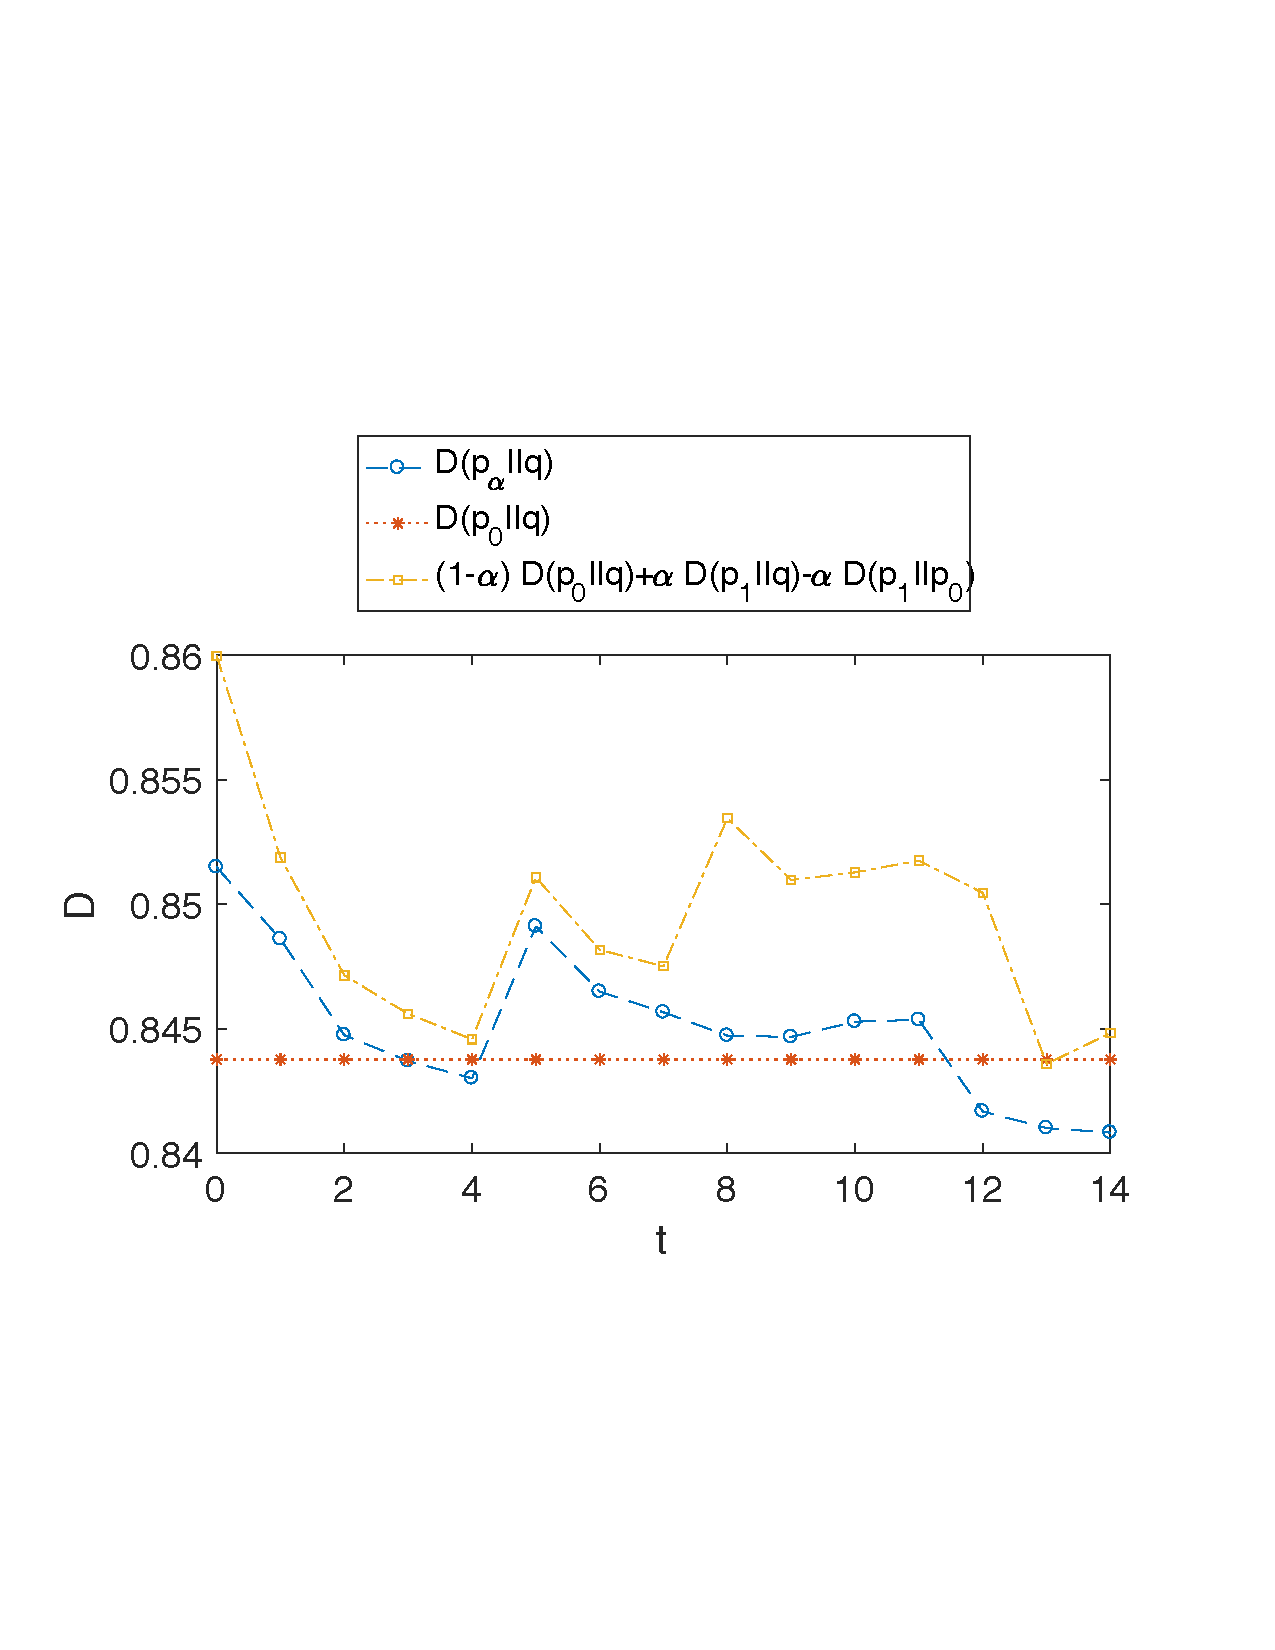
\includegraphics[scale=0.5]{figures/experiment1.pdf}
\caption{Privacy risk $D$ between a user's profile $p$ in the Facebook dataset and reference population distribution $q$.}
\label{fig:7}
\end{figure}

\begin{figure}[htb]
\centering
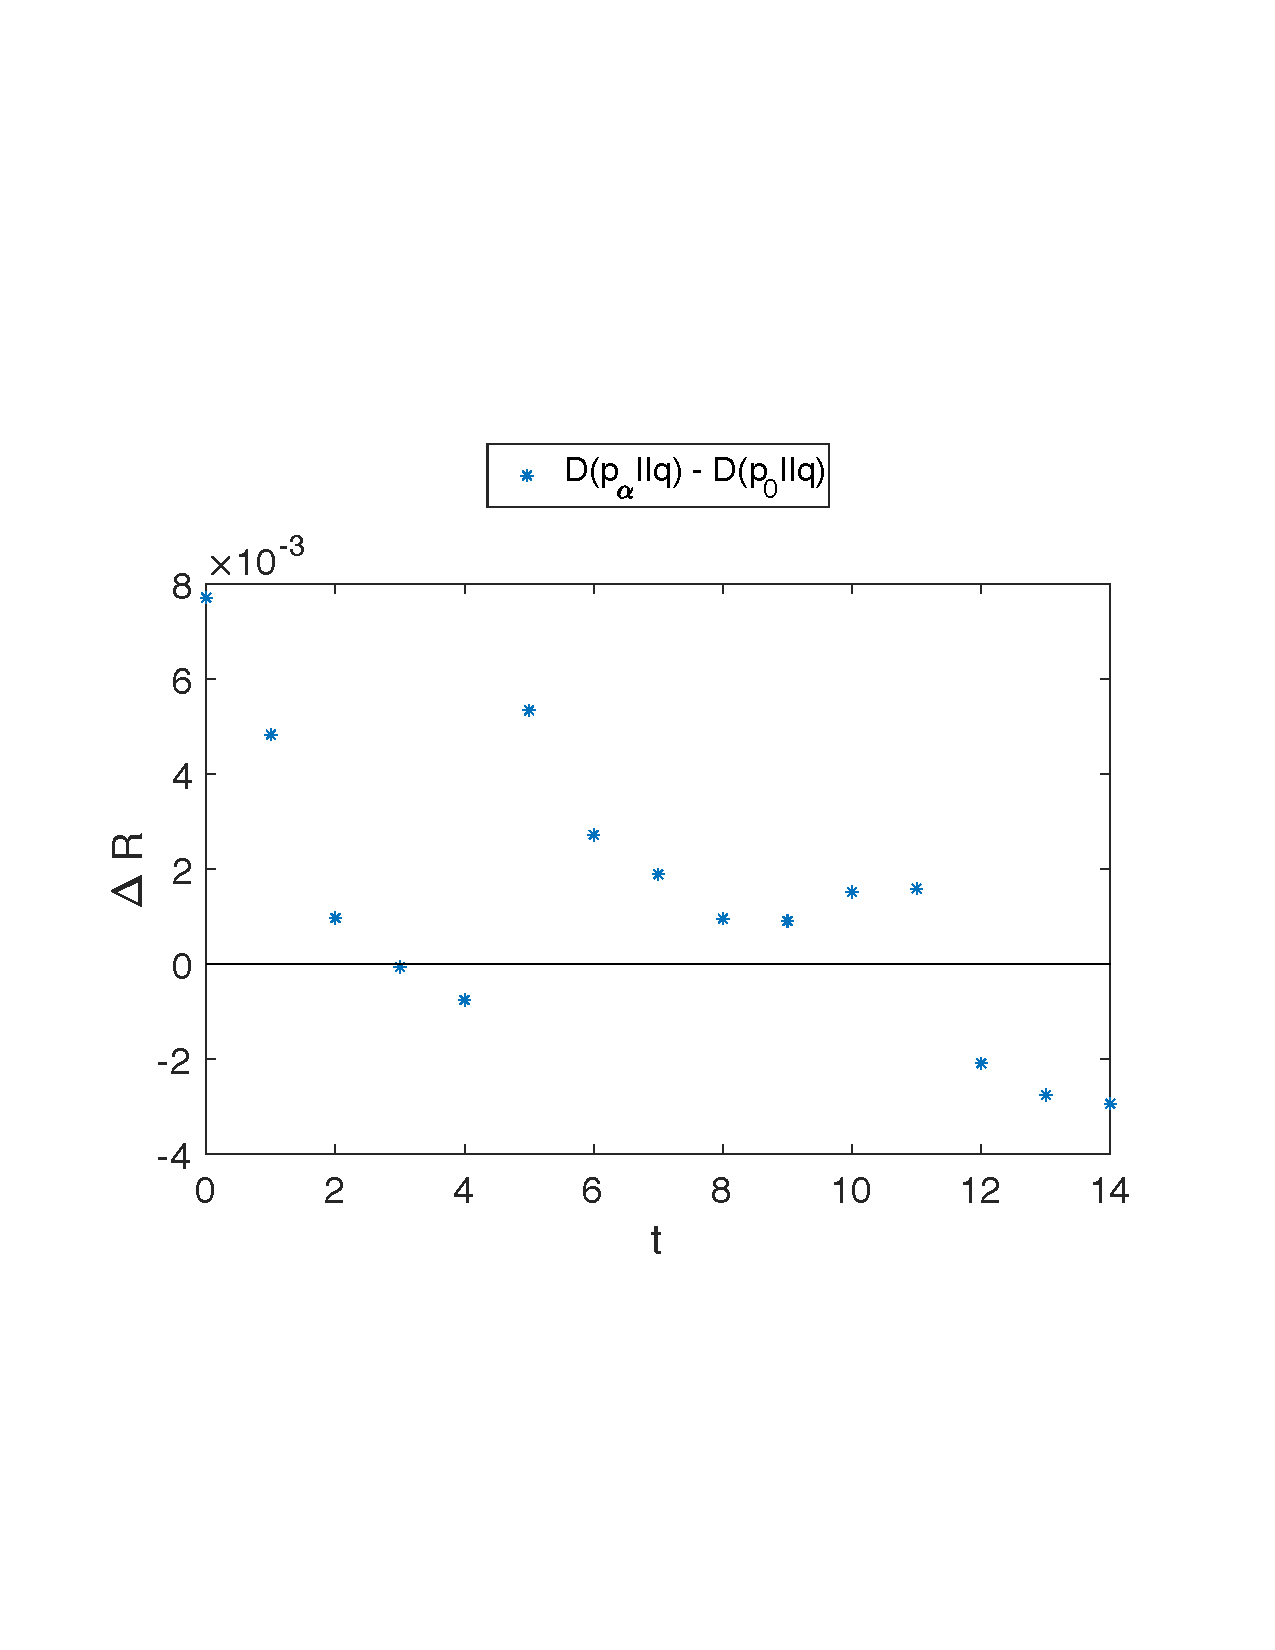
\includegraphics[scale=0.5]{figures/experiment2.pdf}
\caption{$\delta \mathcal{R} = \text{D}(p_\alpha\|q) - \text{D}(p_0\|q)$ where $p_0$ is a user's profile in the Facebook dataset and $q$ is the reference population distribution calculated for all the posts in the dataset.}
\label{fig:8}
\end{figure}


%%%%%%%%%%%%%%%%%%%%%%%%%%%%%%%%%%%%%%%%%%

\section{Discussion}

We introduced two examples (Figures: ~\ref{fig:3}, ~\ref{fig:4}) where we showed how the activity parameter $\alpha$ can be used to estimate a best and worst profile update leading to a new anonymity risk. We computed the analysis both for the divergence (Figure: ~\ref{fig:3}) as well as for the entropy case (Figures: ~\ref{fig:4}). This result is considered relevant especially for practical applications where a user might want to decide their preferred anonymity strategy.

These following examples (Figures: ~\ref{fig:5}, ~\ref{fig:6}) complete the previous ones, presenting the problem of finding a desired profile update, with a fixed activity parameter. Therefore, for a fixed activity parameter $\alpha$ we considered a profile updated leading to the best and worst anonymity risk. We computed the examples both for the divergence (Figure: ~\ref{fig:5}) as well as for the entropy case (Figure: ~\ref{fig:6}).

In our experimental scenario (Figures: ~\ref{fig:7}, ~\ref{fig:8}) we consider a population of users sharing posts on Facebook. The data for this setup is obtained by analysing their time-lines. In Figure: ~\ref{fig:7}, we consider the privacy risk between a user profile and a reference population distribution. This experiments confirm the theoretical analysis and examples presented. Furthermore, we considered (Figure: ~\ref{fig:8}) the privacy risk deltas between the user profile and an updated profile given by a certain activity over time. The experiment shows how a certain activity can theoretically result in an anonymity risk gain or loss.

Note that the theoretical analysis and results proposed in this articles apply to dynamic profiles that change over time. This aspect is particularly interesting, since we are not simply considering profiles as a snapshot of the user's activity, but we are also taking into account changes in interests and general behaviour over time, or consider in a small interval.

Another interesting observation is the fact that profiles might have different privacy risk in different moments of time. This result confirm the intuitive assumption that individuals might change their tastes and interests compared to a reference population. In this case we assume that individuals' profile might change more rapidly over time that a population distribution.

To conclude on the contribution of this chapter, we proposed a series of refinements of a recent information-theoretic model of a user profile expressed through a histogram of categories of interest. The corresponding privacy risk is therefore measured as the Kullback-Leibler divergence with respect to the histogram accounting for the interests of the overall population. Loosely speaking, this risk may be interpreted as an anonymity risk, in the sense that the interests of a specific user may diverge from those of the general population.

Furthermore, we investigate the profile updates leading to the best and worst overall anonymity risk for a given activity and history. Thus, we connect the best case to the fairly recent information-theoretic framework of optimised query forgery and tag suppression for privacy protection.

Hence, we analyse of our model can be applied to an experimental scenario, using Facebook timelines data. Our main objective was measuring how privacy is affected when new content is posted. In fact a user of some on-line service is not able \emph{to know} how much a possible attacker can find out about them. We used real Facebook data to show how our model can be applied on a real world scenario. This aspect is particularly important for Facebook content filtering. In fact, as users are profiled on Facebook, their same activity is used to filter the information they are able to access, based on their interests. There is no transparency on Facebook's side about how this filtering and profiling happens. We hope that studies like this might encourage users to seek more transparency in the filtering techniques used by on-line services.
